%%%%%%%%%%%%%%%%%%%%%%%%%%%%%%%%%%%%%%%%%%%%%%%%%%%%%%%%%%%%%%%%%%%%%%%%%%%

\documentclass{standalone}

\usepackage{amsmath}
\usepackage{mathptmx}
\usepackage{pgfplots}
\usetikzlibrary{external}
\tikzexternalize{water}
\pgfplotsset{compat=1.15}

%% IEEE uses Times Roman font, so we'll default to Times.
%% These three commands make up the entire times.sty package.
\renewcommand{\rmdefault}{ptm}
\renewcommand{\ttdefault}{pcr}
\normalfont\selectfont

\begin{document}

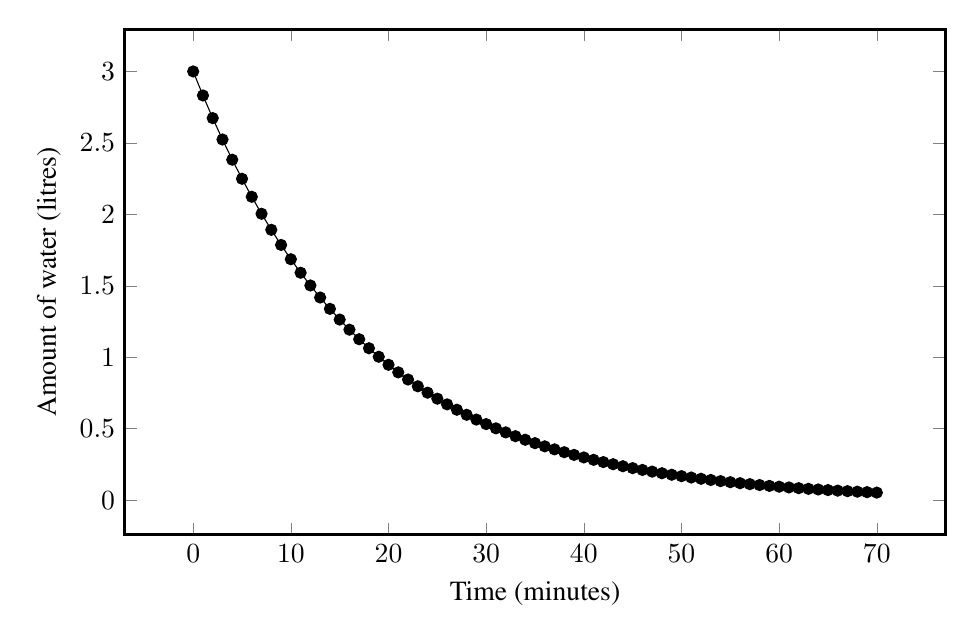
\begin{tikzpicture}
\tikzset{%%
  every mark/.append style={scale=1.0},%%
  scale=1.0%%
}
\pgfplotsset{%%
  every axis/.append style={font=\normalsize}%%
}
%%
\begin{axis}[%%
  axis line style=very thick,%%
  dotStyle/.style={mark size=2,black,mark color=black,mark=*},%%
  enlargelimits=true,%%
  height=8cm,%%
  width=12cm,%%
  %% x axis
  xlabel={\normalsize Time~(minutes)},%%
  %% y axis
  ylabel={\normalsize Amount of water~(litres)},%%
  scaled y ticks=false,%%
  y tick label style=/pgf/number format/fixed%%
]
%%
%%
\addplot[dotStyle] coordinates {
  (0, 3.000000)
  (1, 2.832000)
  (2, 2.673408)
  (3, 2.523697)
  (4, 2.382370)
  (5, 2.248957)
  (6, 2.123016)
  (7, 2.004127)
  (8, 1.891896)
  (9, 1.785950)
  (10, 1.685936)
  (11, 1.591524)
  (12, 1.502399)
  (13, 1.418264)
  (14, 1.338842)
  (15, 1.263866)
  (16, 1.193090)
  (17, 1.126277)
  (18, 1.063205)
  (19, 1.003666)
  (20, 0.947461)
  (21, 0.894403)
  (22, 0.844316)
  (23, 0.797035)
  (24, 0.752401)
  (25, 0.710266)
  (26, 0.670491)
  (27, 0.632944)
  (28, 0.597499)
  (29, 0.564039)
  (30, 0.532453)
  (31, 0.502635)
  (32, 0.474488)
  (33, 0.447917)
  (34, 0.422833)
  (35, 0.399155)
  (36, 0.376802)
  (37, 0.355701)
  (38, 0.335782)
  (39, 0.316978)
  (40, 0.299227)
  (41, 0.282470)
  (42, 0.266652)
  (43, 0.251720)
  (44, 0.237623)
  (45, 0.224316)
  (46, 0.211755)
  (47, 0.199896)
  (48, 0.188702)
  (49, 0.178135)
  (50, 0.168159)
  (51, 0.158742)
  (52, 0.149853)
  (53, 0.141461)
  (54, 0.133539)
  (55, 0.126061)
  (56, 0.119002)
  (57, 0.112338)
  (58, 0.106047)
  (59, 0.100108)
  (60, 0.094502)
  (61, 0.089210)
  (62, 0.084214)
  (63, 0.079498)
  (64, 0.075046)
  (65, 0.070844)
  (66, 0.066876)
  (67, 0.063131)
  (68, 0.059596)
  (69, 0.056259)
  (70, 0.053108)
};
\end{axis}
\end{tikzpicture}

\end{document}
